%%%%%%%%%%%%%%%%%%%%%%%%%%%%%%%%%%%%%%%%%%%%%%%%%%%%%%%%%%%%%%%%%%%%%%%%%%%%%%%
% Análisis en una variable
%
% Copyright (c) 2016 Damián Silvestre. Permission is granted to copy, 
% distribute and/or modify this document under the terms of the 
% GNU Free Documentation License, Version 1.3 or any later version published by
% the Free Software Foundation; with no Invariant Sections, no 
% Front-Cover Texts, and no Back-Cover Texts. 
%
% Details of the GNU FDL can be found here: 
% http://www.gnu.org/licenses/licenses.html
%
%%%%%%%%%%%%%%%%%%%%%%%%%%%%%%%%%%%%%%%%%%%%%%%%%%%%%%%%%%%%%%%%%%%%%%%%%%%%%%%
 
\part{Análisis en una variable}

%%%%%%%%%%%%%%%%%%%%%%%%%%%%%%%%%%%%%%%%%%%%%%%%%%%%%%%%%%%%%
\chapter{Topología en la recta real}

\section{Recta real}

Recordar las propiedades que definen al conjunto de los números reales (ver \ref{numeros_reales}), que también llamaremos recta real por su representación gráfica.

\begin{figure}[h]
\centering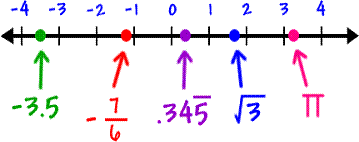
\includegraphics[scale=0.6]{images/03_analisis1/number_line.png}
\caption{Recta real}
\end{figure}

\begin{definition}[Entorno] \label{entorno_real}
Dados $x_0 \in \RR$ y $r > 0$ 
	
Llamamos \textbf{entorno} \index{Recta real!Entorno} (o entorno abierto) de centro $x_0$ y radio $r$ al conjunto
	
$$ E(x_0,r) = \{ x \in \RR^n : d(x,x_0) < r\} $$
	
Llamamos \textbf{entorno cerrado} de centro $x_0$ y radio $r$ al conjunto
	
$$ E[x_0,r] = \{ x \in \RR^n : d(x,x_0) \leq r\} $$
	
Llamamos \textbf{entorno reducido} de centro $x_0$ y radio $r$ a 
	
$$ E'(x_0,r) = E(x_0,r) - \{x_0\}$$
\end{definition}


\begin{definition}[Puntos] \label{clasif_topo_puntos_r}
	
Sea $A \subseteq \RR$, y $x \in \RR$, entonces decimos que $x$ respecto de $A$ es 
	
\begin{itemize}
\item \textbf{Punto interior}: Si existe $E(x,\delta) \subseteq A$.
		
\item \textbf{Punto exterior}: Si existe $E(x,\delta) \subseteq \RR^n - A$.  Equivalentemente $E(x,\delta) \cap A = \emptyset$.
		
\item \textbf{Punto frontera}: Si no es punto interior ni exterior.  Es decir que para todo $ \delta > 0$ se tiene $E(x,\delta) \cap A \neq \emptyset$ y $E(x,\delta) \cap (\RR - A) \neq \emptyset$
		
\item \textbf{Punto clausura} (o adherencia): Si existe un entorno tal que $E(x,r) \cap A \neq \emptyset$
		
\item \textbf{Punto de acumulación} (o punto límite): Si para todo entorno del punto, $ E(x,r) \cap (A - \{x\}) \neq \emptyset$.
		
Equivalentemente, si para todo entorno reducido del punto, $ E'(x,r) \cap A \neq \emptyset$
		
\item \textbf{Punto aislado}: Si existe un entorno tal que $E(x,r) \cap A = \{x\}$
\end{itemize}
\end{definition}

\begin{definition}[Interior] \label{conjunto_interior_r}
Sea $A \subseteq \RR$.  Entonces definimos
	
El \textbf{interior de $A$} como el conjunto de sus puntos interiores, lo denotamos $A^{\circ}$
	
La \textbf{clausura de $A$} como el conjunto de sus puntos de clausura, lo denotamos $\overline{A}$
	
El \textbf{conjunto derivado de $A$} como el conjunto de todos sus puntos de acumulación, lo denotamos $A'$
\end{definition}

%%%%%%%%%%%%%%%%%%%%%%%%%%%%%%%%%%%%%%%%%%%%%%%%%%%%%%%%%%%%%
\chapter{Límite de funciones reales}

\begin{definition}[Límite] \label{limite_r}
Sea $f : A \subset \RR \to \RR$, $ a \in A'$, y $L \in \RR$.  Se dice que el \textbf{límite de $f$ cuando $x$ tiende a $a$} \index{Continuidad!Límite} es $L$ si se cumple cualquiera que:

Para todo $\epsilon > 0$ existe $\delta > 0$ tal que si $x \in A$, $0 < |x-a| < \delta$ entonces $|f(x) - L| < \epsilon$

y en ese caso escribimos

$$ \displaystyle \lim_{x \to a} f(x) = L $$
\end{definition}

\enrojo{Escribir sobre límites laterales, propiedades de límites, infinitésimos equivalentes}

\begin{theorem}[Cero por acotada] \label{cero_por_acotada}
Sean $f,g:A \subseteq \RR \to \RR$, $a \in A'$.

Si $f$ es infinitésimo en $a$ (es decir $ \lim_{x \to a} f(x) = 0$), y $g$ es acotada (es decir $g(A)$ un conjunto acotado) entonces

$$ \lim_{x \to a} f(x)g(x) = 0 $$
\end{theorem}


\section{Asíntotas}


\begin{definition}[Asíntotas]
Sea $f: A \subseteq \RR \to \RR$

\begin{itemize}
\item Sea $x_0 \in A'$.  Si existe alguno de los siguientes límites 

$\lim_{x \to x_0ˆ+} f(x) = \pm \infty$

$\lim_{x \to x_0ˆ-} f(x) = \pm \infty$

decimos que la recta $x = x_0$ es una \textbf{asíntota vertical de $f$}.


\item Si existe alguno de los siguientes límites 

$\lim_{x \to \pm \infty} f(x) = k \in \RR$ 

decimos que $y = k$ es asíntota horizontal de $f$.


\item Si existen $a,b \in \RR$, tales que existe algunos de los siguientes límites

$\lim_{x \to \pm \infty} f(x) - (ax+b) = 0$ 

decimos que $y = ax+b$ es asíntota oblicua de $f$.

Para calcular $a$ y $b$ (si existen) primero se calcula el siguiente límite

$ a = \lim_{x \to \pm \infty} \frac{f(x)}{x} $

y luego conociendo $a$ se calcula el siguiente límite

$ b = \lim_{x \to \pm \infty} f(x) - ax $
\end{itemize}
\end{definition}


%%%%%%%%%%%%%%%%%%%%%%%%%%%%%%%%%%%%%%%%%%%%%%%%%%%%%%%%%%%%%
\chapter{Funciones contínuas}

Recordar la definición de intervalo de números reales (ver \ref{intervalo}).

\enrojo{Definir compacto, conexo, 
demostrar que compacto de R equivale a cerrado y acotado,
demostrar que continuas mandan compactos en compactos y conexos en conexos.  
Demostrar que intervalo equivale a conexo.
}

\begin{theorem}[Bolzano]
Sea $f : A \subseteq \RR \to \RR$ contínua en $[a,b] \subseteq A$, con $f(a) f(b) < 0$ (es decir tal que $f(a)$ y $f(b)$ tienen signo opuesto).

Entonces existe $c \in [a,b]$ tal que $f(c) = 0$ (es decir existe una raíz)
\end{theorem}

\begin{proof}
Como $[a,b] \subseteq \RR$ es cerrado y acotado, es compacto.  Como $f$ es contínua, $f([a,b])$ es compacto.

Como $[a,b]$ es un intervalo, es conexo.  Como $f$ es contínua, $f([a,b])$ es conexo, es decir es un intervalo.

Luego $f([a,b])$ es un intervalo compacto, es decir cerrado y acotado.

Como es un intervalo, y como $f(a), f(b) \in f([a,b])$, para todo $d$ entre $f(a)$ y $f(b)$ se tiene que $d \in f([a,b])$.  En particular como $f(a)$, $f(b)$ tienen signo opuesto, uno de esos $d$ es el $0$.

En otras palabras, existe $c \in [a,b]$ tal que $f(c) = 0$. 
\end{proof}



%%%%%%%%%%%%%%%%%%%%%%%%%%%%%%%%%%%%%%%%%%%%%%%%%%%%%%%%%%%%%
\chapter{Funciones diferenciables}

\begin{definition}[Derivada] \label{derivada}
Una función $f : A \subset \RR \to \RR$ es derivable en $x_0 \in A^{\circ}$ si existe el siguiente límite

$$ f'(x_0) = \lim_{h \to 0} \frac{f(x_0 + h) - f(x_0)}{h} $$

En ese caso decimos que $f'(x_0)$ es la derivada de $f$ en $x_0$.
\end{definition}

\begin{definition}[Recta tangente]
Sea $f : A \subset \RR \to \RR$ derivable en $x_0 \in A^{\circ}$.  Sea $y_0 = f(x_0)$

Entonces la \textbf{recta tangente a $f$ en $x_0$} es

$ y - y_0 = f'(x_0) (x - x_0)$

Y la \textbf{recta normal a $f$ en $x_0$} es

$ y - y_0 = \frac{-1}{f'(x_0)} (x - x_0)$
\end{definition}

\begin{observation}[Álgebra de deriv]

Sean $f,g : A \subseteq \RR \to \RR$ funciones derivables.  

Entonces

$(f(x) \pm g(x))' = f'(x) \pm g'(x)$

$(k f(x))' = k f'(x) $ para todo $k \in \RR$

$(f(x) \cdot g(x))' = f'(x) g(x) + f(x) g'(x)$

$(f(x) / g(x))' = \frac{ f'(x) g(x) - f(x) g'(x) }{ gˆ2(x) }$
\end{observation}

\begin{theorem}[Regla de la cadena] \label{regla_cadena} 

Sean

$ f : A \subset \RR \to \RR$ diferenciable en $x_0 \in A^{\circ}$

$ g : B \subset \RR \to \RR$ diferenciable en $y_0 = f(x_0) \in B^{\circ}$

tales que $f(A) \subseteq B$

Entonces la función compuesta $h : A \to \RR$ es diferenciable en $x_0$, y además 

$$ h'(x_0) = g'(f(x_0)) \cdot f'(x_0) $$
\end{theorem} 

Tabla de derivadas de algunas funciones

\begin{center}
\begin{tabular}{|c|c|}
\hline
$f(x)$ & $f'(x)$ \\
\hline
$k$ & $0$ \\
\hline
$xˆn$ & $n xˆ{n-1}$ \\
\hline
$eˆx$ & $eˆx$ \\
\hline
$\cos(x)$ & $-\sin(x)$ \\
\hline
$\sin(x)$ & $\cos(x)$ \\
\hline
$\tan(x)$ & $\frac{1}{\cosˆ2(x)}$ \\
\hline
$\arccos(x)$ & $\frac{-1}{ \sqrt{1 - xˆ2} }$ \\
\hline
$\arcsin(x)$ & $\frac{1}{ \sqrt{1 - xˆ2} }$ \\
\hline
$\arctan(x)$ & $\frac{1}{1 + xˆ2}$ \\
\hline
\end{tabular}
\end{center}

\enrojo{Agregar mas funciones a la tabla.  Definir derivadas laterales, y punto anguloso.}

El siguiente teorema se generaliza en Cálculo de varias variables (ver \ref{dif_impl_cont}).

\begin{theorem}[Deriv impl. cont] \ref{deriv_impl_cont}
Sea $ f : A \subset \RR \to \RR$ derivable en $ x_0 \in A^{\circ}$.

Entonces $f$ es contínua en $x_0$.
\end{theorem}

\begin{proof}
Como $f$ es derivable en $x_0$, existe

$f'(x_0) = \lim_{x \to x_0} \frac{f(x) - f(x_0)}{x - x_0}$

Queremos calcular el siguiente límite

$ \lim_{x \to x_0} f(x) - f(x_0)$

$ = \lim_{x \to x_0} \frac{f(x) - f(x_0)}{x - x_0} (x - x_0)$

$ = f'(x_0) 0 = 0$

Luego

$ \lim_{x \to x_0} f(x) = f(x_0)$

es decir $f$ es contínua en $x_0$.
\end{proof}

\begin{definition}[Sucesivas]
Sea $f:A \subseteq \RR \to \RR$.

Sea $A_1 \subseteq A$ el conjunto de puntos donde $f$ es derivable.  Definimos la función derivada primera como $f' : A_1 \to \RR$, $x \to f'(x)$.

Sea $A_2 \subseteq A_1$ el conjunto de puntos donde $f'$ es derivable.  Definimos la función derivada sucesiva segunda como $f'' : A_2 \to \RR$, $x \to f''(x)$.

Siguiendo así, sea $A_k$ el conjunto de puntos donde $fˆ{(k-1)}$ es derivable.  Definimos la función \textbf{derivada sucesiva $k$-ésima} como $fˆ{(k)} : A_k \to \RR$, $x \to fˆ{(k)}(x)$

Si $A$ abierto, decimos que \textbf{$f$ es clase $Cˆk$} y escribimos $f \in Cˆk$ si las derivadas hasta orden $k$ existen y son contínuas en $A$.
\end{definition}

\begin{theorem}[Inversa]
Sea $f : A \subseteq \RR \to \RR$ biyectiva y derivable con $f'(x) \neq 0$, $\forall x \in A$.

Digamos que $y = f(x)$.

Entonces $f^{-1}$ es derivable y $f^{-1}'(y) = \frac{1}{f'(x)}$

\end{theorem}

\begin{proof}

\enrojo{Demostramos sólo la fórmula, asumiendo que $f^{-1}$ es derivable.}

Como son inversas, tenemos que

$f^{-1}(f(x)) = x$

Aplicando la regla de la cadena

$f^{-1}'(f(x)) f'(x) = 1$

Es decir

$f^{-1}'(y) = \frac{1}{f'(x)}$
\end{proof}



%%%%%%%%%%%%%%%%%%%%%%%%%%%%%%%%%%%%%%%%%%%%%%%%%%%%%%%%%%%%%
\chapter{Aproximación de funciones por polinomios}

%%%%%%%%%%%%%%%%%%%%%%%%%%%%%%%%%%%%%%%%%%%%%%%%%%%%%%%%%%%%%
%\chapter{Integral indefinida}

%%%%%%%%%%%%%%%%%%%%%%%%%%%%%%%%%%%%%%%%%%%%%%%%%%%%%%%%%%%%%
\chapter{Cálculo integral}

%%%%%%%%%%%%%%%%%%%%%%%%%%%%%%%%%%%%%%%%%%%%%%%%%%%%%%%%%%%%%
\chapter{Relaciones entre el cálculo diferencial e integral}

%%%%%%%%%%%%%%%%%%%%%%%%%%%%%%%%%%%%%%%%%%%%%%%%%%%%%%%%%%%%%
\chapter{Sucesiones, series numéricas y funcionales}



